\chapter{Introduction}

People re-identification (Re-ID) has been an intense research topic in recent years, whose main goal is to match a given person with those persons with known labels. Person Re-ID has great potential in video surveillance, target detection and tracking and forensic search. However, it is quite challenging since the accuracy is much influenced by many factors like occlusion, illumination variation, camera settings and color response. In Re-ID, those images with known labels are called gallery images and the image used to know its label is called probe image. The probe image and gallery images can be from the same or different camera views, so the viewpoint and illumination between probe and gallery image can be quite different. Also for the different color response of different cameras, the shots of the same person may look different in different cameras. Besides, occlusions between camera and target person can also bring about quite much difficulty.  In a word, images of the same person may look different while images of different persons may kook quite the same. 

Given a sequence or video of individuals, there are three steps to match person. A simple work flow is shown in figure \ref{workflow}. However, since most of used Re-ID datasets are well copped manually or by a automatic detector, so most Re-ID work will only focus on robust descriptors designing and efficient matching algorithm designing aimed at those well cropped images. 


\begin{figure}[]
\centering
\begin{raggedleft}
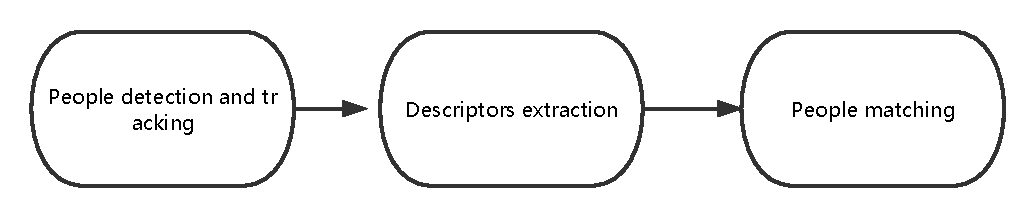
\includegraphics[scale = 0.8]{/Users/JohnsonJohnson/Downloads/thesis_1/Figures/REIDframework.pdf}
%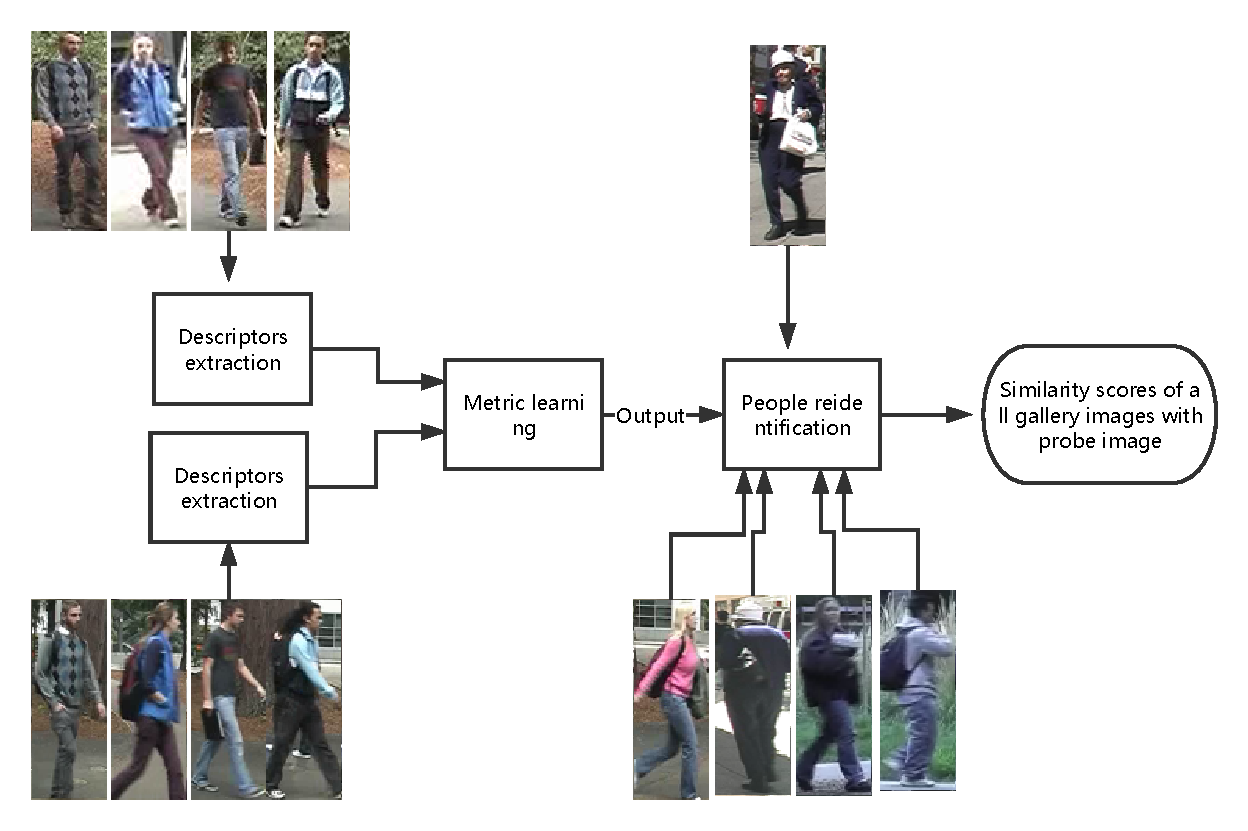
\includegraphics[width=1\linewidth]{REIDworkflow.pdf}
\vspace{1em}
\caption{Re-ID work flow}
\end{raggedleft}
\end{figure}
\label{workflow}

\begin{figure}[H]
\centering
%\begin{raggedleft}
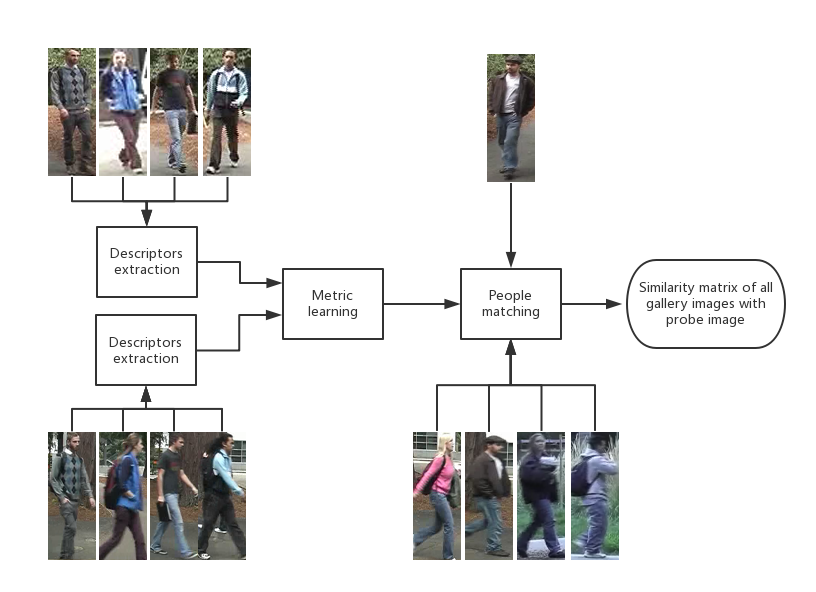
\includegraphics[scale = 0.5]{/Users/JohnsonJohnson/Downloads/thesis_1/Figures/REIDworkflow.png}
%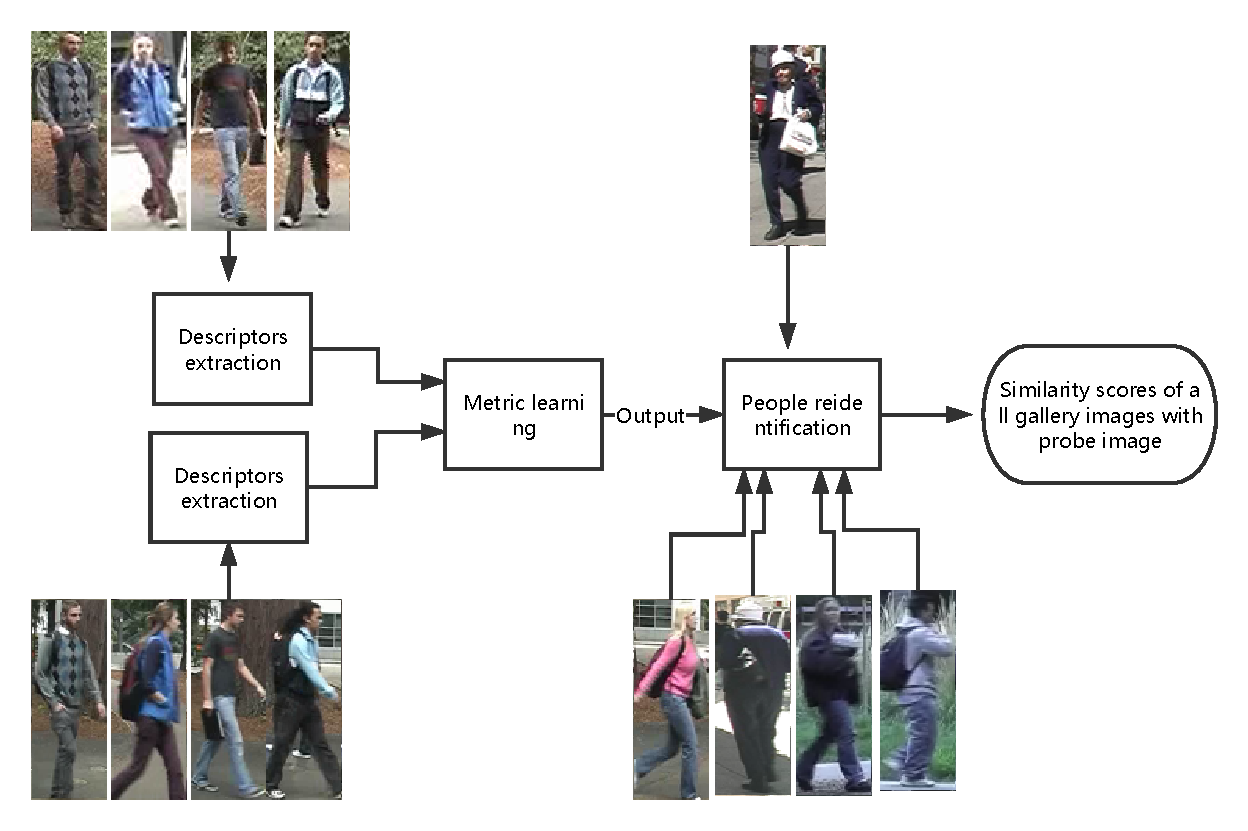
\includegraphics[width=1\linewidth]{REIDworkflow.pdf}
\vspace{1em}
\caption{A typical single shot Re-ID work flow}
%\end{raggedleft}
\end{figure}




The first task in Re-ID is to design a robust descriptor to represent images. The descriptor is supposed to contain the key information for each captured person. Basically, the descriptors are supposed to be robust and discriminative. One straightforward way is to extract the color, textural information of images, then the descriptors are used to compute the similarity score. But this method turns out to be not robust caused by illumination variation  and camera color response difference and camera angle settings.  Therefore, many other advanced descriptors takes into account the correlation of color, texture and position together to improve performance.


The second one is to design the similarity computing methodology. That is, the way to compare how similar two descriptors are. Previous methods use Euclidean distance, Bhattacharyya distance and Mahalanobis distance. The Euclidean distance is the easiest to match descriptors like color and texture descriptors. However, though it's straightforward and easy, it's hard to use Euclidean distance to discriminate images. 
Many creative metric learning methods have been proposed to compute descriptor similarity. Among them the Mahanalobis distance based metric is most popular. In this method a semi-positive defined matrix $\bm{M}$ is learned while meeting certain intraclass and interclass distance limitations. Besides, linear discriminant analysis \cite{LFDA} learns a subspace to minimize the within class scatter matrix while maximized inter class scatter matrix. In \cite{NFST} the null space is proposed that make descriptors of same class collapse into a single point while descriptors of different classes are projected to different points. 
	
\section{Basic concepts}
People re-identification can be divided into a few categories according to different conditions. Some general concepts are listed below.\\
\indent \textbf{Open set and close set Re-ID} \cite{REIDsurvey} According gallery size and if the gallery size evolves, Re-ID can be divided in to open set Re-ID and close set Re-ID. In close set Re-ID, no new identities will be added to gallery set and gallery size remains the same as time goes by. Besides, the probe set will be a subset of gallery set, that means, the number of unique identities in gallery set will be equal or greater than probe set. In open set Re-ID, the gallery set will evolve as time goes by. Each time a probe image is inputed to the recognition system, the system will judge if it has a corresponding match in the gallery set. If the probe image doesn't match any of the gallery images, it will be regarded as a new identity and will be added to the gallery set. Besides, the probe set is not necessarily the subset of gallery set. 

\textbf{Long term and short term Re-ID} According to the time interval between gallery and probe images, Re-ID can be divided into long term and short term Re-ID.  In short term means the time interval between gallery and probe images are small, say a few minutes or several hours. In contrary, the long term Re-ID refers to the case that the time interval between gallery and probe images are a few days or even longer. The difference brought by long time interval between gallery and probe images is the variation of individuals' clothes and appearance. If the gallery images are shot a few days ago, the same individual may have changes his suits or take off his bag, then the appearance may change a lot. In this case, it will be much more difficult to recognize the same identity in long term Re-ID. Generally, in most cases we use the short term Re-ID, which guarantees the appearance of same person will remain the same and we only need to consider the difference brought by other factors like viewpoint variation and occlusions.


\textbf{Single shot and multi shot Re-ID} According to the size of sample set for each person, Re-ID can be divided into single shot and multi shots approaches. In single shot case, only one image is provided for a person in a camera view. Single shot Re-ID is challenging because only limited information can be extracted. One example is the VIPeR dataset figure \ref{VIPeRimages}, in this dataset, for each person only one image is provides in each camera view and the viewpoint of each view is different. In multi shots Re-ID a sequence of images are provided for a person in a camera view. Compared with single shot case, more extra information, like temporal-spatial can be extracted from the sample set. One case of multi-shot dataset is the prid\_2011 dataset which provides a long sequence for each person in a single camera view.

%-------------------------------------------------
\begin{figure}[H]

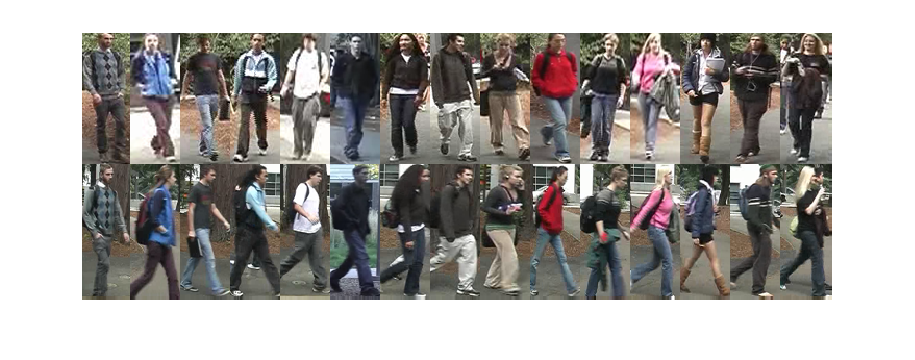
\includegraphics[width=1\linewidth]{/Users/JohnsonJohnson/Downloads/thesis_1/Figures/singleREID.eps}
\vspace{-3em}
\caption{The VIPeR dataset}
\label{VIPeRimages}
\end{figure}

%-------------------------------------------------

\begin{figure}[H]

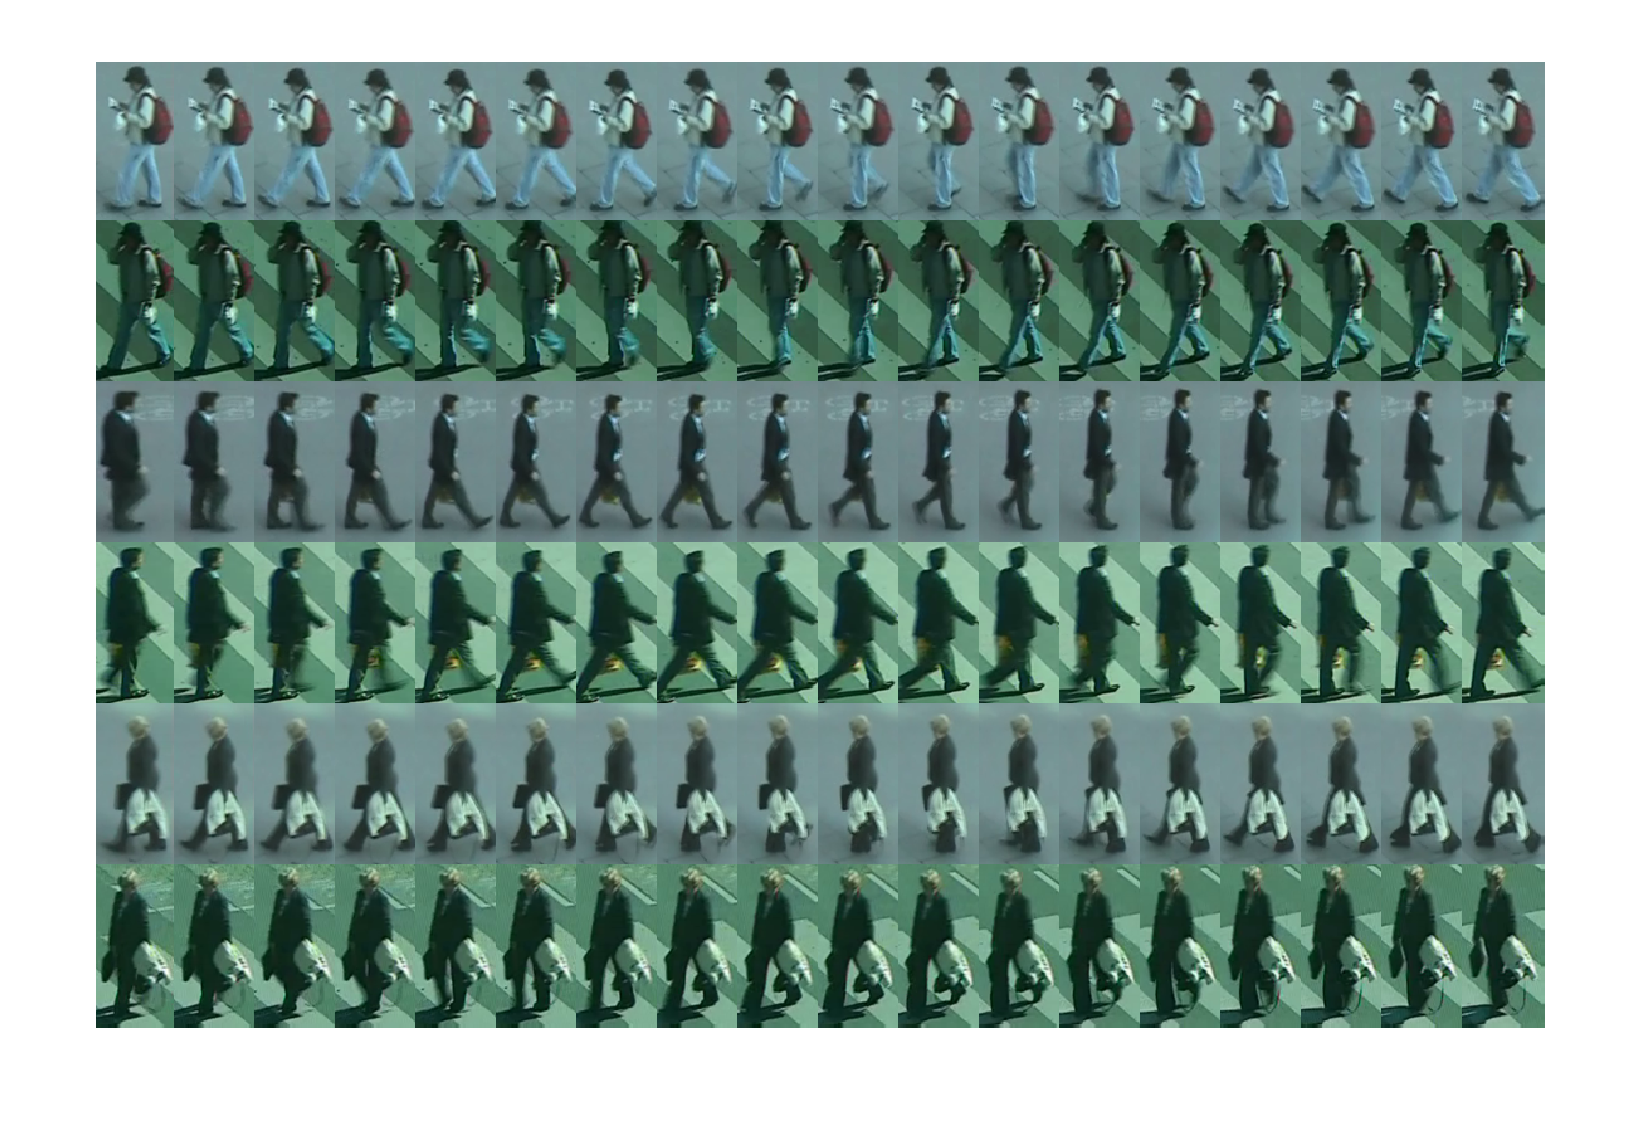
\includegraphics[width=1\linewidth]{/Users/JohnsonJohnson/Downloads/thesis_1/Figures/Multishots.eps}
\vspace{-3em}
\caption{Samples from prid\_2011 dataset}

\end{figure}


.

\section{Challenges}

\textbf{Detection, tracking and dataset labelling for supervised learning} Though classical person re-identification focus on descriptors designing and matching designing, in real-time application the detection and tracking has to be operated on video frames to get well cropped bounding box images. A good detection and tracking algorithm is necessary for Re-ID. Besides, training the matching algorithm is supervised process, thus we have to know the labels for those training data. Manual labelling turns to be unrealistic for large size dataset. So it's vital to design a automatic labelling algorithm.

\textbf{Descriptors designing} Good descriptors should be robust to people pose variation, outer environment changes and camera settings. Though there have been many kinds of descriptors based on different property like color and texture, it's hard to judge which property is a universally useful for different camera settings. In fact, the robustness, reliability and feasibility depends quite much on different camera settings. What's more, the pedestrian background may bring about much error to descriptors, so it's important to quantify the impact of noisy background. Many works have tried to use segmented foreground of pedestrians, so it's important to design segmentation algorithms. The automatic foreground segmentation for single frame is quite tough since there isn't that much available information compared with video background segmentation. Take VIPeR dataset as an example, there is only one frame for each view of a certain person, thus the segmented foreground masks are imperfect and chance is high that important body parts are lost. A segmented foreground provided by \cite{SDALF} is shown is figure \ref{VIPeRFG}.
%-------------------------------------------------
\begin{figure}[H]
\centering
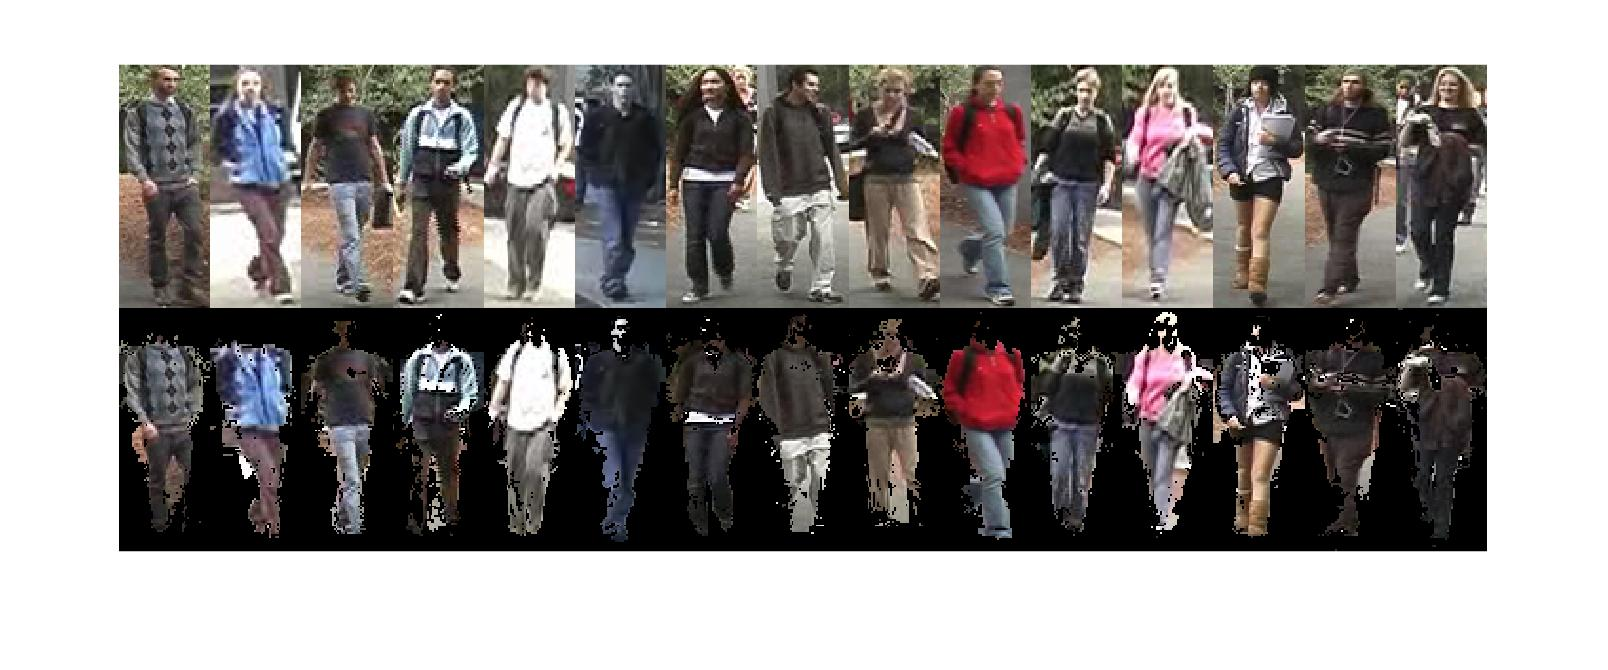
\includegraphics[width=1\linewidth]{/Users/JohnsonJohnson/Downloads/thesis_1/Figures/FGdemo.jpg}
\vspace{-3em}
\caption{VIPeR foreground}
\label{VIPeRFG}
\end{figure}

%-------------------------------------------------
\textbf{Efficient matching algorithm designing} 	
When designing machine learning algorithms to match persons, there are many limitations. One of them is the small sample size problem \cite{NFST}. The extracted descriptors usually has a high dimension $d$ but only a small number of sample $n(n<<d)$ size are available, underfitting may appear for insufficient data samples with high dimension. Besides, it's also necessary to have a good consideration of intra and inter distance of samples.
The intra distance means the distance of two samples with the same class label, while inter class distance is the distance of samples with different class labels. 

\textbf{Feasibility, Complexity and Scalability} When applying those descriptors and matching algorithms, we have to consider the its real-time performance.   The Re-ID datasets usually has small sample size but in surveillance network much more pedestrians in different cameras can be presented simultaneously. A system like this has plenty of individuals to re-identify, which requires the process time for single probe should be short for low latency. Besides, the since the gallery in this system evolves, it's crucial to design a evolution algorithm for gallery images, that is, how to judge if a person appeared in current camera is a new person to all those gallery images.

\section{Proposed work}
In many previous work, the kernel local fisher discriminant analysis is used as a subspace learning method, and Euclidean distance is usually used in the subspace to measure similarity. In this thesis, the KLFDA \cite{KLFDA} method is used a dimension reducing method to project high dimensional descriptors to a lower dimension space. Compared with other dimension reduction methods, KLFDA is a supervised method and it takes consideration of those intra and inter class information, therefore, much less information are lost after dimension reduction. Then a Mahanalobis distance based matrix $M$ is learned based on the limitation that the distance of people from same class should be at least 1 unit smaller than the distance of people from different classes. A target function that penalizes large intra-class distance and small inter-class distance is created, by iterative computation, when the target function converges the matrix $M$ is thought to be optimal. It turns out that this metric learning have advance performance when compared with other metric learning methods. A workflow of proposed work is in figure \ref{ProposedWorkflow}.

%------------------------------------------------------------
\begin{figure}[H]

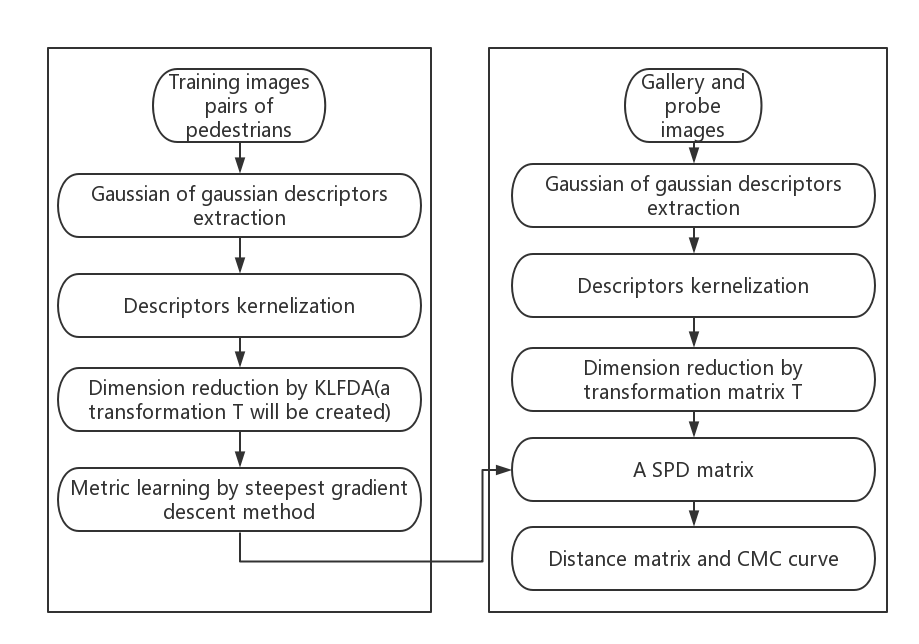
\includegraphics[width=1\linewidth]{/Users/JohnsonJohnson/Downloads/thesis_1/Figures/ProposedWorkFlow.png}
\vspace{-2em}
\caption{The workflow of proposed work}
\label{ProposedWorkflow}

\end{figure}
%------------------------------------------------------------
\begin{figure}[H]

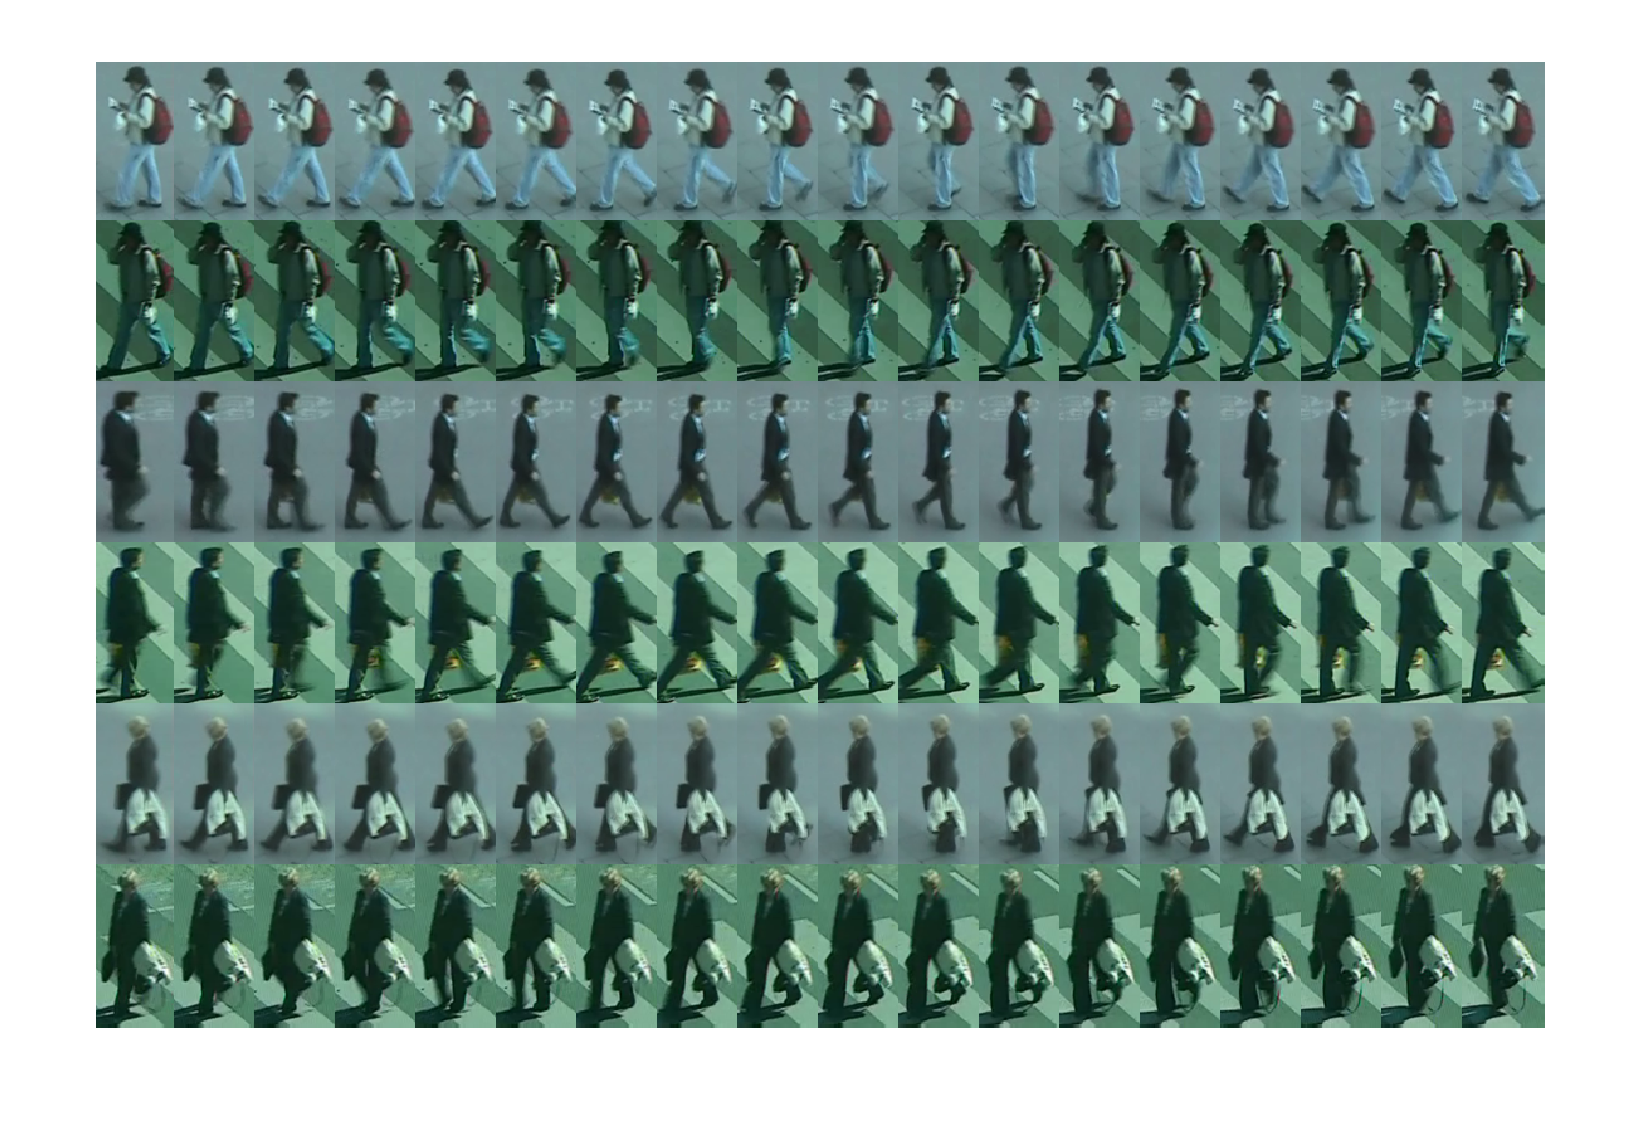
\includegraphics[width=1\linewidth]{/Users/JohnsonJohnson/Downloads/thesis_1/Figures/Multishots.eps}
\vspace{-2em}
\caption{Samples from prid\_2011 dataset}

\end{figure}


\section{Performance measuring}

There are a few measures of Re-ID, such as cumulative matching curve(CMC) curve and Receiver Operating Characteristic curve(ROC) curve. Specifically, CMC is used as a 1:m reidentification system and ROC is used for 1:1 reidentification system.  In this thesis, the cumulative matching curve is used to measure Re-ID performance. The $CMC(k)$  stands for the probabilty that the right match is within the top k matches. Suppose a set of gallery $G = \{G_1,G_2,\cdots,G_m\}$ and a set of probe $P = \{P_1,P_2,\cdots,P_n\}$, for each identity $P_i$ there should be a right match in the gallery set. However, there could be identities that appear in gallery set but not in probe set. A $m\times n$ similarity matrix can be computed. Then for each probe identity $P_i$, a sorted list of gallery identities can be list as $S(P_i) = \{{G_{1},G_{2},\cdots,G_{m}}\}$ so that their similarity with $P_i$ descends. Suppose the right match of $P_i$ is at the position $k$ of $S(P_i)$, $k\le m$, then $G_i$ has a rank value of $k$. Therefore, the CMC can be calculated as 
\begin{equation}
CMC(k) = \frac{1}{n}(\#k_l\le k)
\end{equation}
where $k_l$ is the list of rank values of $P = \{P_1,P_2,\cdots,P_n\}$, and $\#k_l\le k$ means the number of rank values that is smaller than k.  Therefore, CMC curve always ascends and stops at 1.  A perfect CMC curve is supposed to have a hight rank 1 score and approaches 1 as fast as possible.




\section{Contribution}

In this paper we have two contributions, the first is we combined the KLFDA with distance comparison learning. Instead of learning the subspace with KLFDA and computing Euclidean distance in lower dimensional space, a Mahanalobis distance based matrix is learned under the limitation that the within class distance is at least 1 unit smaller than inter class distance. Compared with those advanced metrics including cross view quadratic analysis(XQDA) \cite{LOMO} and Null space learning(NFST), this proposed metric learning proves to have excellent performance on VIPeR, CUHK1, prid\_2011, prid\_450s and GRID dataset.

Another contribution of this thesis is the influence of background subtraction on different descriptors are probed. We found that the background subtraction can improve the performance of descriptors (like HSV histogram) but can decrease the performance of  certain descriptors (texture feature like LBP and HOG). This comparison is shown in Chapter 3. The reason for this is imperfect background segmentation brings about textural interference. If descriptors are color based and don't handle texture information, like HSV histogram descriptor, background segmentation can greatly improve the performance. However, if the descriptor extracts texture information, background segmentation will decrease its performance since the imperfect segmentation will cause many small black dots in foreground area, which will cause gigantic textural information variation. Because segmentation algorithm will cause different influence on various features, in this thesis, a weighted map of images is used instead of using the background segmentation.

\section{Thesis organization}
In this thesis, Chapter 2 will give a brief introduction of previous work. Chapter 3 will explain the implementation of the hierarchical gaussian descriptors used in this thesis. In Chapter 4 a detailed introduction of the kernel local fisher local discriminant analysis will be presented, and a detailed explanation will also be presented about the metric learning on the lower dimension space based on relative distance limitation learning.
In Chapter 5 the used datasets and parameters and other experiment settings will be explained, and a detailed analysis of results is presented here. At last, the conclusion is given in Chapter 6.




